\documentclass[a4paper, 12pt]{article}

\usepackage[left=1.5cm, right=1.5cm, top=1.5cm, bottom=1.5cm]{geometry}
\usepackage{graphicx}
\usepackage{xcolor}
\usepackage{mdframed}
\usepackage { amsmath , amssymb , amsthm }
\usepackage[T2A]{fontenc}
\usepackage[utf8]{inputenc}
\usepackage[english,russian]{babel}
\usepackage{listings}
\usepackage{setspace}
% \usepackage{indentfirst} 
\singlespacing 

\lstset{language=SQL,
  basicstyle={\small\ttfamily},
  belowskip=3mm,
  breakatwhitespace=true,
  breaklines=true,
  classoffset=0,
  columns=flexible,
  commentstyle=\color{dkgreen},
  framexleftmargin=0.25em,
  frameshape={}{yy}{}{}, %To remove to vertical lines on left, set `frameshape={}{}{}{}`
  keywordstyle=\color{blue},
  numbers=none, %If you want line numbers, set `numbers=left`
  numberstyle=\tiny\color{gray},
  showstringspaces=false,
  stringstyle=\color{green},
  tabsize=3,
  xleftmargin =1em
}

\graphicspath{{img/}}
\DeclareGraphicsExtensions{.pdf,.png,.jpg}


\begin{document}
\begin{titlepage}
  \begin{center}
    \MakeUppercase{Министерство науки и высшего образования Российской Федерации} \\
    \MakeUppercase{ФГБОУ ВО Алтайский госудаственный университет}
    \vspace{0.25cm}
    
	  Институт цифровых технологий, электроники и физики
    
    Кафедра вычислительной техники и электроники
    \vfill
    
    {\LARGE Лабораторные работы, 13 вариант}\\[5mm]
    \textsc{(Отчёт по лабораторным работам по курсу <<Методы оптимизации>>)}
  \bigskip

\end{center}
\vfill

\newlength{\ML}
\settowidth{\ML}{«\underline{\hspace{0.7cm}}» \underline{\hspace{1cm}}}
\hfill
\begin{minipage}{0.45\textwidth}
  Выполнил ст. 3-го курса, 595 гр.:\\
  \underline{\hspace{\ML}} Д.\,В.~Осипенко\\
  Проверил: преп. каф. ВТиЭ\\
  \underline{\hspace{\ML}} Я.\,С.~Сергеева\\
  «\underline{\hspace{0.7cm}}» \underline{\hspace{2cm}} \the\year~г.
\end{minipage}%
\vfill

\begin{center}
  Барнаул, \the\year~г.
\end{center}
\end{titlepage}
\tableofcontents
\newpage

\section{Графический метод решения задач линейного программирования}
Дана задача:\\

\begin{math}
  Z(X)=2x_1+4x_2 \rightarrow  \text{min} \\
  \begin{cases}
    2x_1-x_2 \geq 0\\
    -x_1-x_2 \leq 0\\
    3x_1+7x_2 \leq 40\\
    8x_1-4x_2 \leq 26\\
  \end{cases}\\
  x_1\geq 0, \quad x_2\geq 0
\end{math}\\

Изобразим на плоскости систему координат $Ox_1x_2$ и построим граничные прямые ОДР:\\

\begin{math}
  x_1\geq 0, \quad x_2\geq 0\\
  \begin{cases}
    2x_1-x_2 \geq 0,(1)\\
    -x_1-x_2 \leq 0,(2)\\
    3x_1+7x_2 \leq 40,(3)\\
    8x_1-4x_2 \leq 26,(4)\\
  \end{cases}\\
\end{math}\\

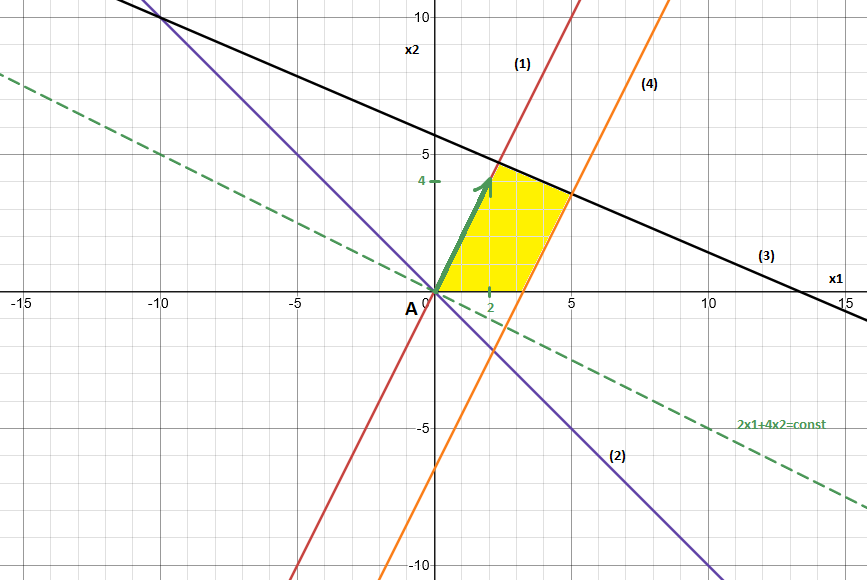
\includegraphics[width=\textwidth]{1-1.png}
\begin{center}
  Рис. 1.1 Область допустимых решений
\end{center}

Для линий уровня $2x_1+4x_2 = \text{const}$ строим нормальный вектор $\vec{n} = (2,4)$ перпендикулярно вектору нормаль построим одну из линий уровня Перемещаем её в направлении вектора $\vec{n}$ до опорной прямой. Для определения координат точки A решаем систему уравнений:\\

\begin{math}
  \begin{cases}
    2x_1-x_2 \geq 0,(1)\\
    -x_1-x_2 \leq 0,(2)\\
  \end{cases}
\end{math}\\

Получаем $x_1 = 0, x_2 = 0$ это и есть оптимальное решение. Минимальное значение целевой функции $Z(X) = 2 \cdot 0 + 4 \cdot 0 = 0$.



% 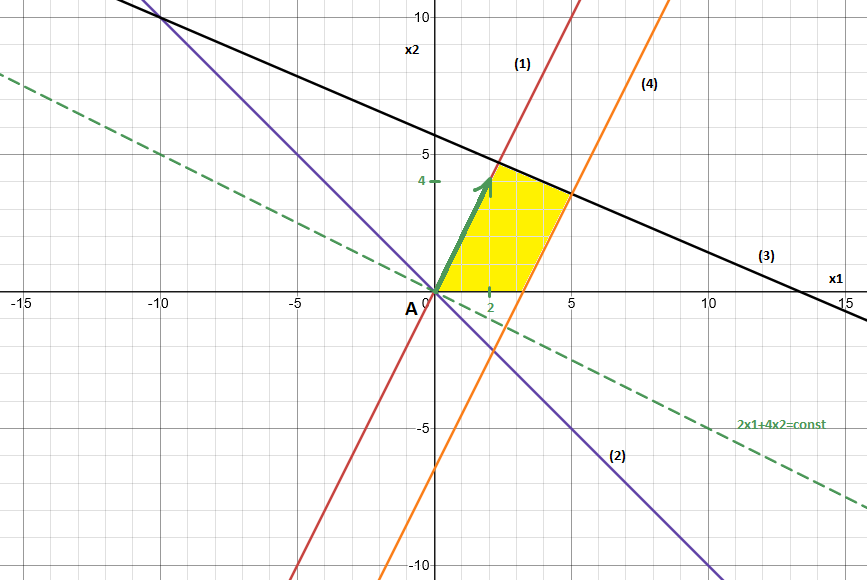
\includegraphics[width=\textwidth]{1-1.png}\\

\end{document}